% Ready-to-\input figure environments for the eval2 set (docs/figures/eval2 -> cvpr2027/figs).
% Not included from main.tex; copy a block into the section where it belongs and edit the caption.

\begin{figure*}[t]\centering
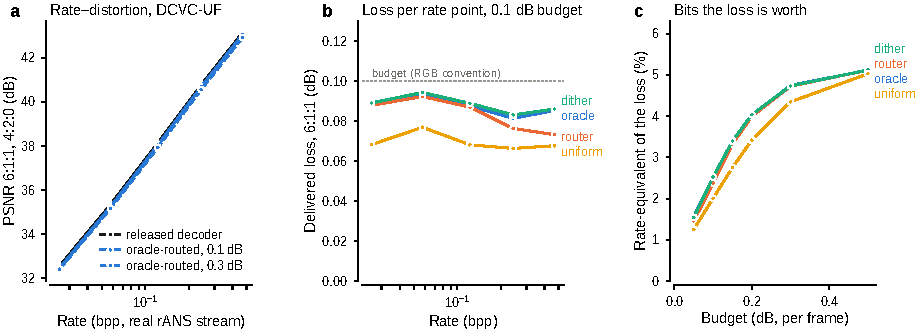
\includegraphics[width=\textwidth]{figs/fig1_rd_bd.pdf}
\caption{DCVC-UF on the 53 CTC intra frames (five qp). (a) Rate--distortion of the released decoder and the oracle-routed decoder at 0.1 and 0.3\,dB budgets (real rANS rate, PSNR 6:1:1 in 4:2:0). (b) Delivered loss per rate point at the 0.1\,dB budget, four selection rules. (c) Rate-equivalent of the delivered loss on the released RD curve, as a function of the budget.}
\label{fig:rd_bd}\end{figure*}

\begin{figure}[t]\centering
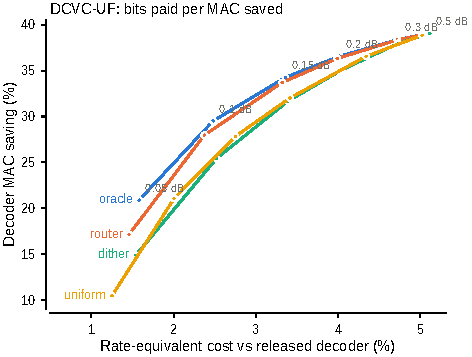
\includegraphics[width=\linewidth]{figs/fig2_bd_frontier.pdf}
\caption{Decoder MAC saving against the rate-equivalent cost of the delivered loss, DCVC-UF, four selection rules; budgets as points.}
\label{fig:bd_frontier}\end{figure}

\begin{figure*}[t]\centering
\includegraphics[width=\textwidth]{figs/fig3_saving_vs_budget.pdf}
\caption{Saving against budget for the four selection rules: DCVC-UF (CTC), NoGAN-MS and ELIC on Kodak-24 and CLIC-41. Means over the frames feasible under every rule at that budget.}
\label{fig:saving_budget}\end{figure*}

\begin{figure*}[t]\centering
\includegraphics[width=\textwidth]{figs/fig4_premium.pdf}
\caption{Adaptivity premium. (a) Oracle minus the best content-blind rule against budget, five datasets. (b) DCVC-UF: oracle$-$dither, router$-$dither and dither$-$uniform.}
\label{fig:premium}\end{figure*}

\begin{figure*}[t]\centering
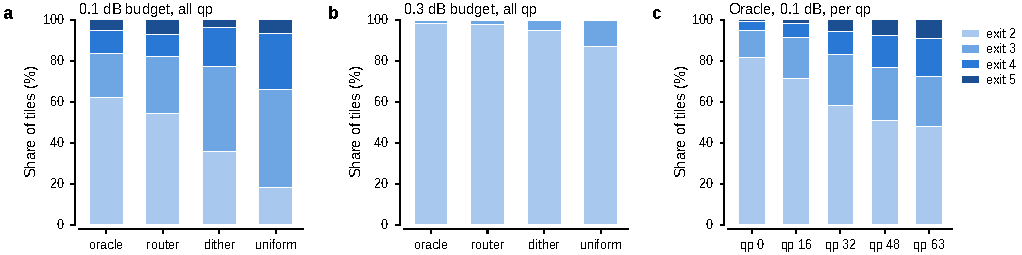
\includegraphics[width=\textwidth]{figs/fig5_exit_usage.pdf}
\caption{Share of tiles per exit, DCVC-UF: the four rules at 0.1\,dB (a) and 0.3\,dB (b); the oracle per qp at 0.1\,dB (c).}
\label{fig:usage}\end{figure*}

\begin{figure*}[t]\centering
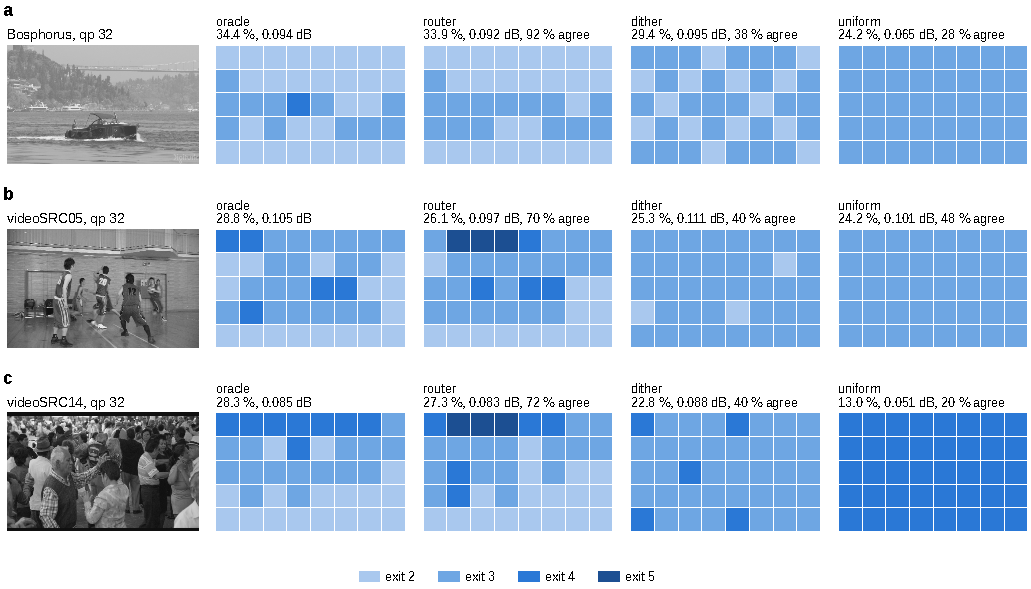
\includegraphics[width=\textwidth]{figs/fig6_maps.pdf}
\caption{Example frames (qp 32) and the exit maps chosen by the four rules at the 0.1\,dB budget, with saving, delivered loss (6:1:1) and agreement with the oracle map.}
\label{fig:maps}\end{figure*}

\begin{figure*}[t]\centering
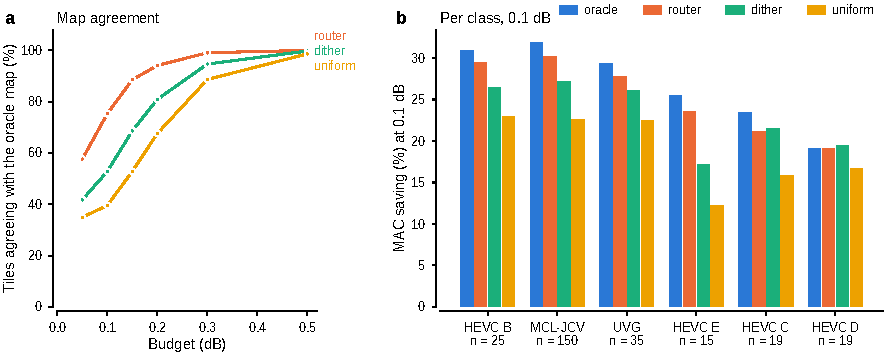
\includegraphics[width=\textwidth]{figs/fig7_agreement_class.pdf}
\caption{(a) Tiles agreeing with the oracle map against budget. (b) Saving per CTC class at 0.1\,dB.}
\label{fig:agreement}\end{figure*}

\begin{figure*}[t]\centering
\includegraphics[width=\textwidth]{figs/fig8_rung_ladders.pdf}
\caption{Uniform rung ladders: dB cost against saving of every uniform configuration, DCVC-UF, NoGAN-MS and ELIC.}
\label{fig:ladders}\end{figure*}

\begin{figure*}[t]\centering
\includegraphics[width=\textwidth]{figs/fig9_per_image.pdf}
\caption{Per-image saving of the content-blind rules against the oracle at 0.1\,dB, Kodak-24 and CLIC-41.}
\label{fig:per_image}\end{figure*}

\begin{figure*}[t]\centering
\includegraphics[width=\textwidth]{figs/fig10_distortion_compute.pdf}
\caption{Delivered loss against saving for the image decoders, four rules, Kodak-24 and CLIC-41.}
\label{fig:distortion_compute}\end{figure*}

\begin{figure*}[t]\centering
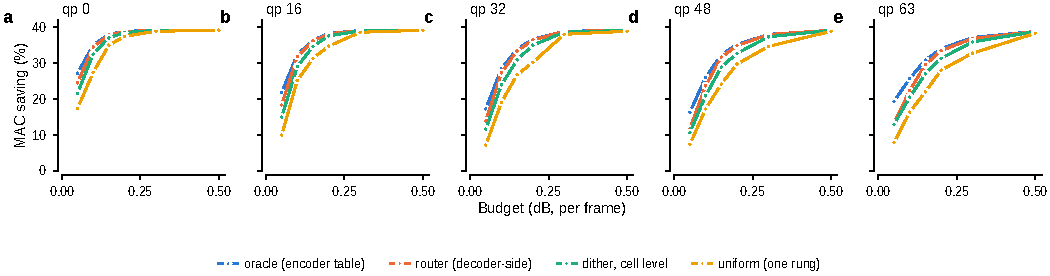
\includegraphics[width=\textwidth]{figs/fig11_dcvcuf_per_qp.pdf}
\caption{DCVC-UF per qp: saving against budget for the four rules, real decodes.}
\label{fig:per_qp}\end{figure*}

% ---- encoder / decoder runtime (cvpr2027/reports/encoder_runtime) ----
\begin{figure*}[t]\centering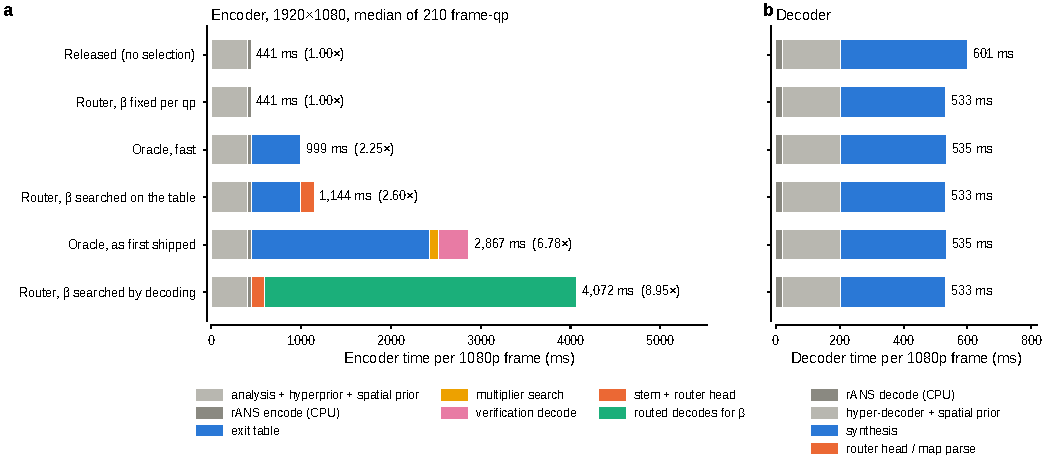
\includegraphics[width=\textwidth]{figs/rt_fig1_timeline_1080p.pdf}
\caption{Encoder (a) and decoder (b) time per 1080p frame for each exit-map selection regime, split into stages (DCVC-UF, CTC).}\label{fig:rt_timeline}\end{figure*}
\begin{figure*}[t]\centering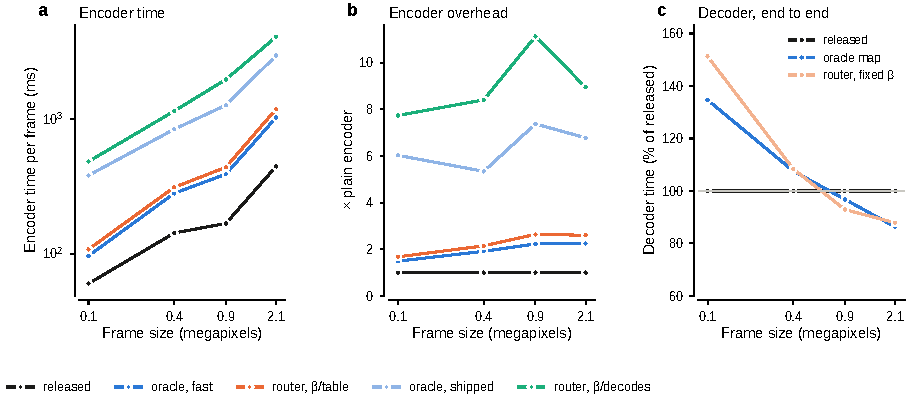
\includegraphics[width=\textwidth]{figs/rt_fig2_resolution.pdf}
\caption{Encoder time (a), encoder overhead (b) and end-to-end decoder time (c) against frame size.}\label{fig:rt_resolution}\end{figure*}
\begin{figure*}[t]\centering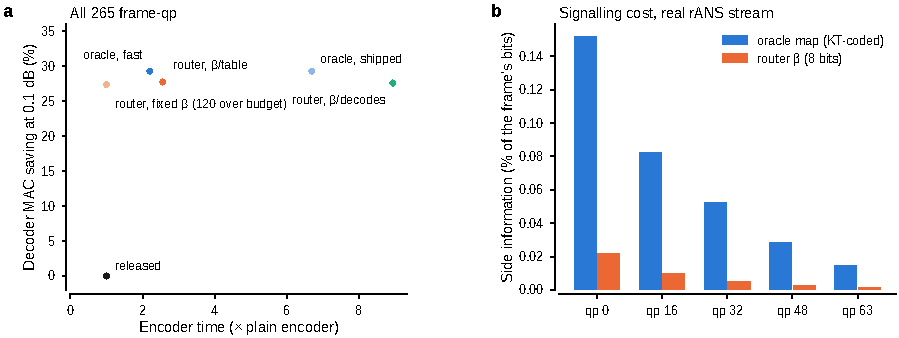
\includegraphics[width=\textwidth]{figs/rt_fig3_tradeoff.pdf}
\caption{Decoder MAC saving against encoder overhead (a) and side information as a share of the real bitstream (b).}\label{fig:rt_tradeoff}\end{figure*}
\begin{figure*}[t]\centering\includegraphics[width=\textwidth]{figs/rt_fig4_image_decoders.pdf}
\caption{Oracle search cost for NoGAN-MS and ELIC (a), saving delivered (b) and decodes per image (c).}\label{fig:rt_image}\end{figure*}
% ---- encoder / decoder runtime (cvpr2027/reports/encoder_runtime) ----
\begin{figure*}[t]\centering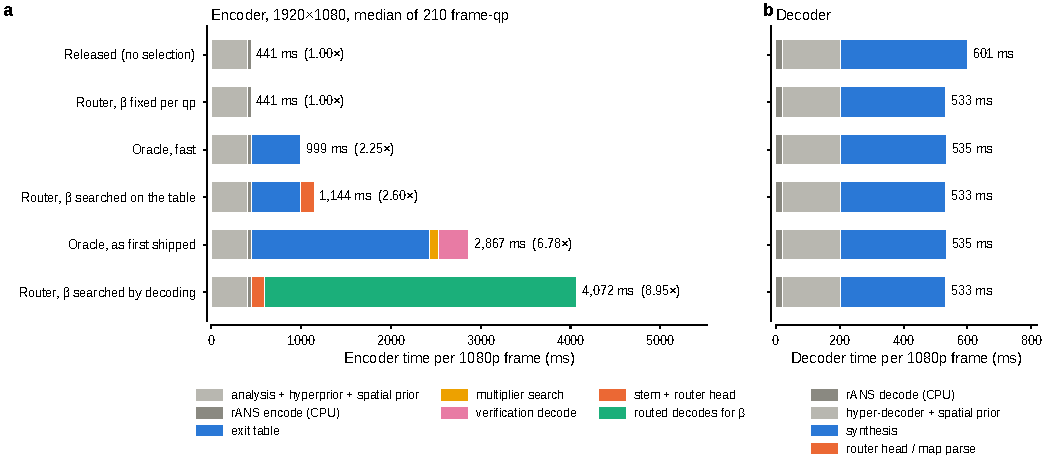
\includegraphics[width=\textwidth]{figs/rt_fig1_timeline_1080p.pdf}
\caption{Encoder (a) and decoder (b) time per 1080p frame for each exit-map selection regime, split into stages (DCVC-UF, CTC).}\label{fig:rt_timeline}\end{figure*}
\begin{figure*}[t]\centering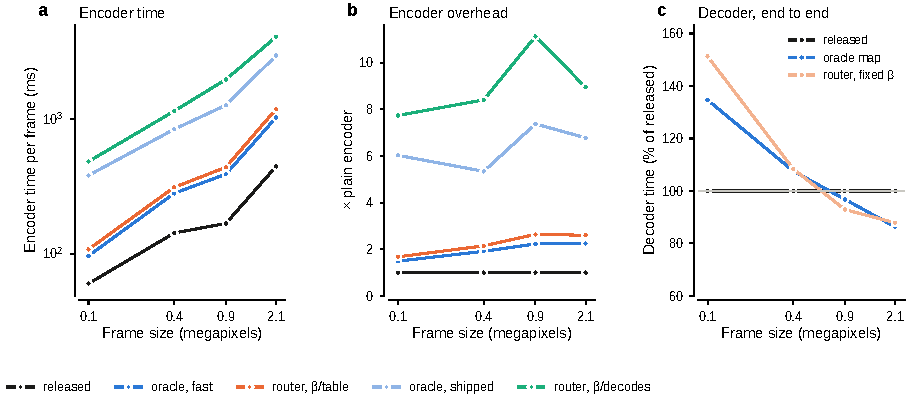
\includegraphics[width=\textwidth]{figs/rt_fig2_resolution.pdf}
\caption{Encoder time (a), encoder overhead (b) and end-to-end decoder time (c) against frame size.}\label{fig:rt_resolution}\end{figure*}
\begin{figure*}[t]\centering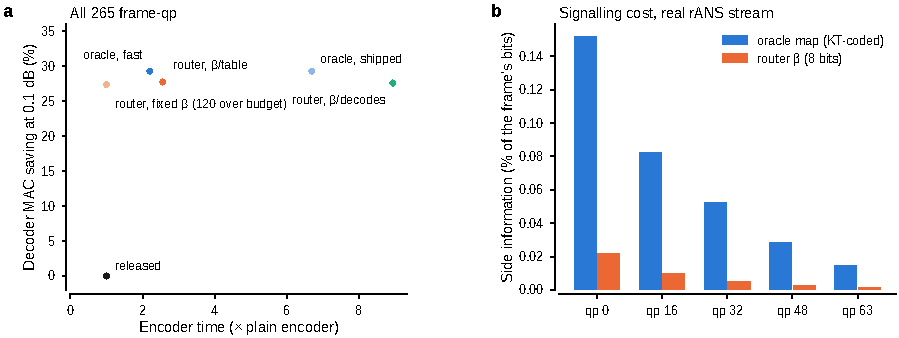
\includegraphics[width=\textwidth]{figs/rt_fig3_tradeoff.pdf}
\caption{Decoder MAC saving against encoder overhead (a) and side information as a share of the real bitstream (b).}\label{fig:rt_tradeoff}\end{figure*}
\begin{figure*}[t]\centering\includegraphics[width=\textwidth]{figs/rt_fig4_image_decoders.pdf}
\caption{Oracle search cost for NoGAN-MS and ELIC (a), saving delivered (b) and decodes per image (c).}\label{fig:rt_image}\end{figure*}
% ---- encoder / decoder runtime (cvpr2027/reports/encoder_runtime) ----
\begin{figure*}[t]\centering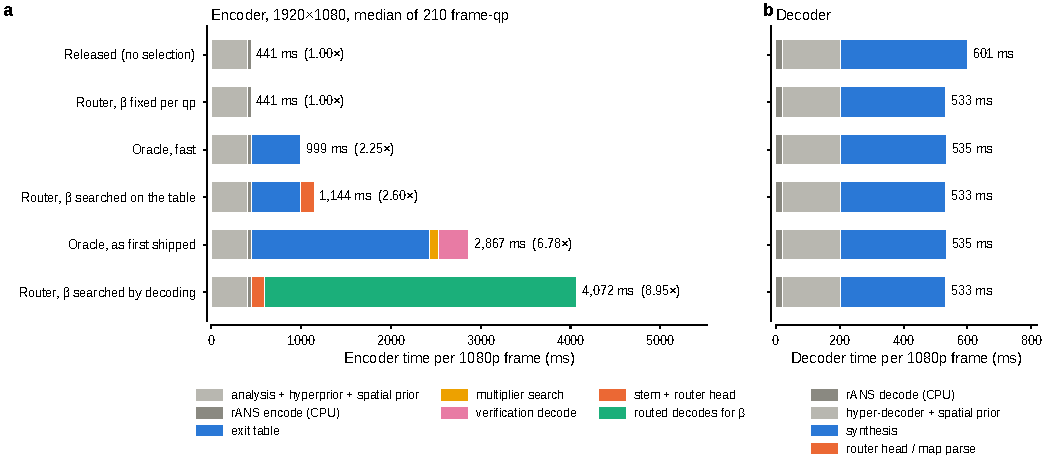
\includegraphics[width=\textwidth]{figs/rt_fig1_timeline_1080p.pdf}
\caption{Encoder (a) and decoder (b) time per 1080p frame for each exit-map selection regime, split into stages (DCVC-UF, CTC).}\label{fig:rt_timeline}\end{figure*}
\begin{figure*}[t]\centering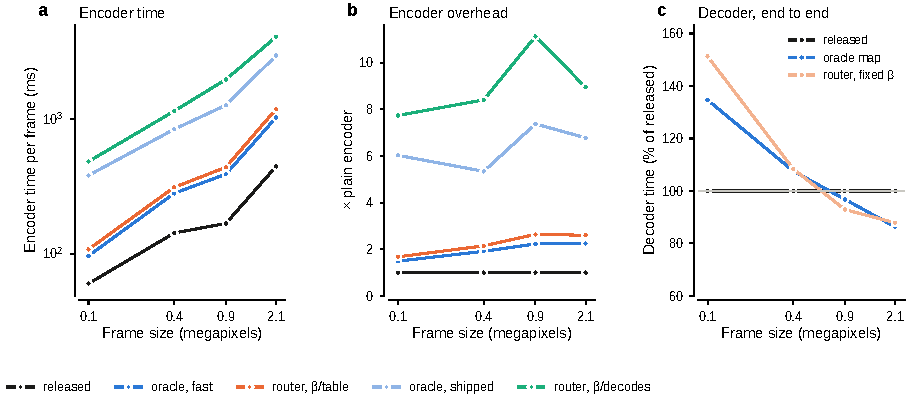
\includegraphics[width=\textwidth]{figs/rt_fig2_resolution.pdf}
\caption{Encoder time (a), encoder overhead (b) and end-to-end decoder time (c) against frame size.}\label{fig:rt_resolution}\end{figure*}
\begin{figure*}[t]\centering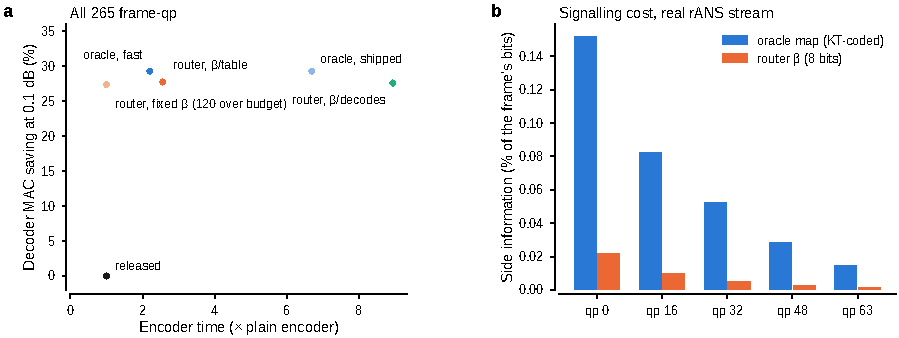
\includegraphics[width=\textwidth]{figs/rt_fig3_tradeoff.pdf}
\caption{Decoder MAC saving against encoder overhead (a) and side information as a share of the real bitstream (b).}\label{fig:rt_tradeoff}\end{figure*}
\begin{figure*}[t]\centering\includegraphics[width=\textwidth]{figs/rt_fig4_image_decoders.pdf}
\caption{Oracle search cost for NoGAN-MS and ELIC (a), saving delivered (b) and decodes per image (c).}\label{fig:rt_image}\end{figure*}
% ---- encoder / decoder runtime (cvpr2027/reports/encoder_runtime) ----
\begin{figure*}[t]\centering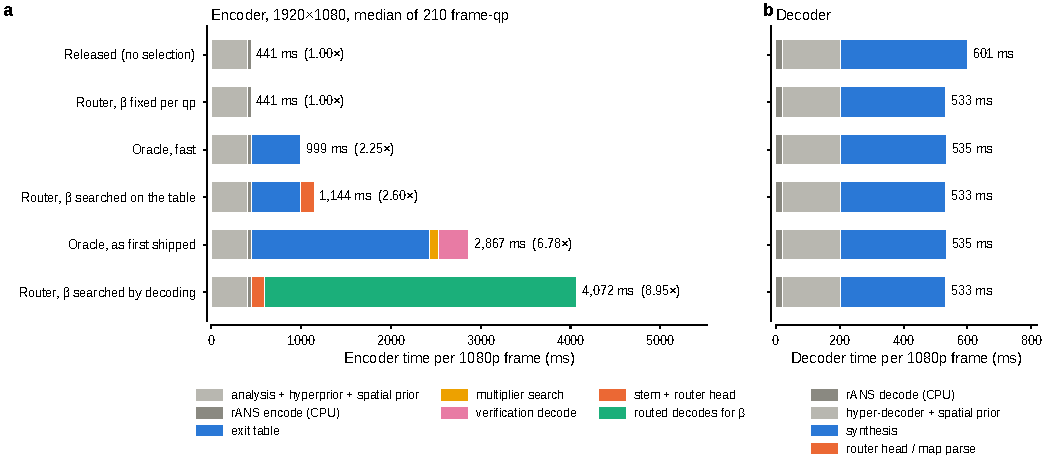
\includegraphics[width=\textwidth]{figs/rt_fig1_timeline_1080p.pdf}
\caption{Encoder (a) and decoder (b) time per 1080p frame for each exit-map selection regime, split into stages (DCVC-UF, CTC).}\label{fig:rt_timeline}\end{figure*}
\begin{figure*}[t]\centering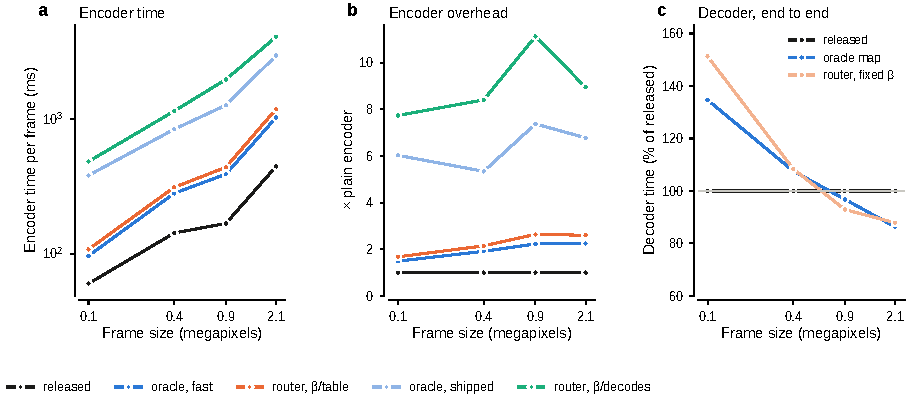
\includegraphics[width=\textwidth]{figs/rt_fig2_resolution.pdf}
\caption{Encoder time (a), encoder overhead (b) and end-to-end decoder time (c) against frame size.}\label{fig:rt_resolution}\end{figure*}
\begin{figure*}[t]\centering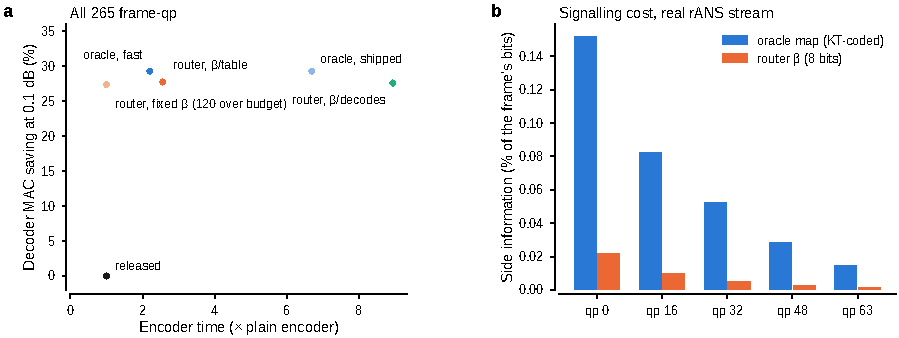
\includegraphics[width=\textwidth]{figs/rt_fig3_tradeoff.pdf}
\caption{Decoder MAC saving against encoder overhead (a) and side information as a share of the real bitstream (b).}\label{fig:rt_tradeoff}\end{figure*}
\begin{figure*}[t]\centering\includegraphics[width=\textwidth]{figs/rt_fig4_image_decoders.pdf}
\caption{Oracle search cost for NoGAN-MS and ELIC (a), saving delivered (b) and decodes per image (c).}\label{fig:rt_image}\end{figure*}
% ---- encoder / decoder runtime (cvpr2027/reports/encoder_runtime) ----
\begin{figure*}[t]\centering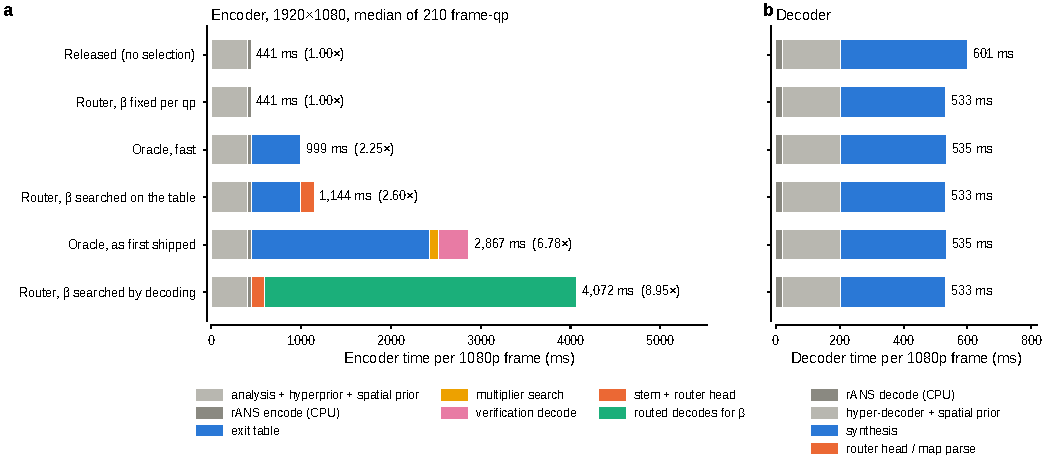
\includegraphics[width=\textwidth]{figs/rt_fig1_timeline_1080p.pdf}
\caption{Encoder (a) and decoder (b) time per 1080p frame for each exit-map selection regime, split into stages (DCVC-UF, CTC).}\label{fig:rt_timeline}\end{figure*}
\begin{figure*}[t]\centering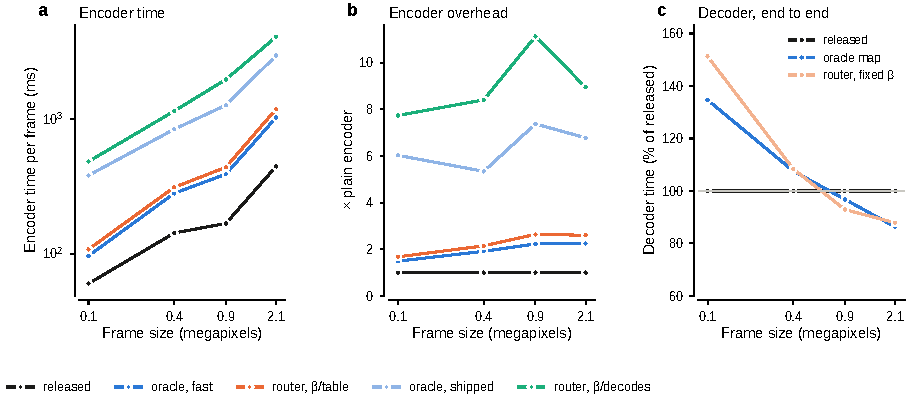
\includegraphics[width=\textwidth]{figs/rt_fig2_resolution.pdf}
\caption{Encoder time (a), encoder overhead (b) and end-to-end decoder time (c) against frame size.}\label{fig:rt_resolution}\end{figure*}
\begin{figure*}[t]\centering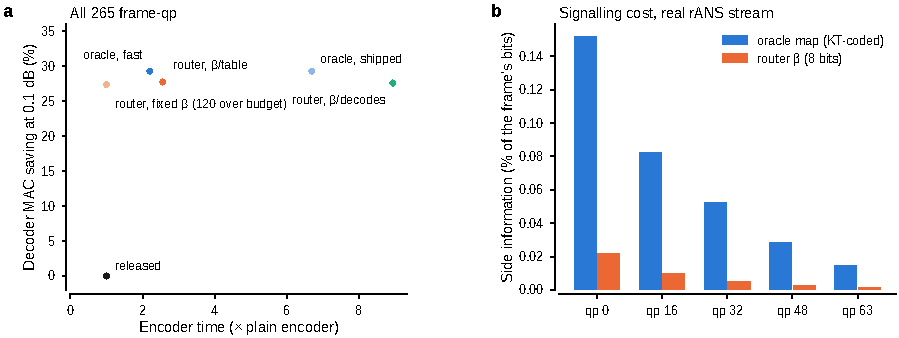
\includegraphics[width=\textwidth]{figs/rt_fig3_tradeoff.pdf}
\caption{Decoder MAC saving against encoder overhead (a) and side information as a share of the real bitstream (b).}\label{fig:rt_tradeoff}\end{figure*}
\begin{figure*}[t]\centering\includegraphics[width=\textwidth]{figs/rt_fig4_image_decoders.pdf}
\caption{Oracle search cost for NoGAN-MS and ELIC (a), saving delivered (b) and decodes per image (c).}\label{fig:rt_image}\end{figure*}
% ---- encoder / decoder runtime (cvpr2027/reports/encoder_runtime) ----
\begin{figure*}[t]\centering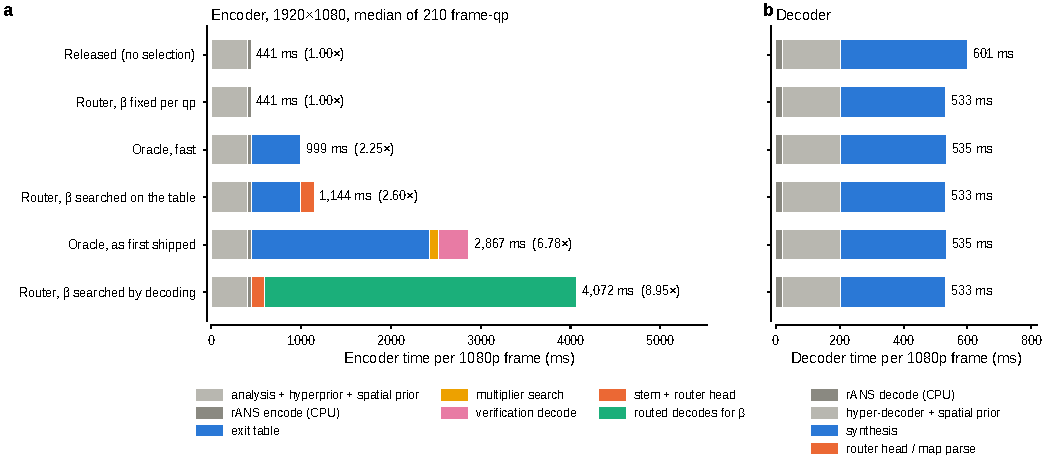
\includegraphics[width=\textwidth]{figs/rt_fig1_timeline_1080p.pdf}
\caption{Encoder (a) and decoder (b) time per 1080p frame for each exit-map selection regime, split into stages (DCVC-UF, CTC).}\label{fig:rt_timeline}\end{figure*}
\begin{figure*}[t]\centering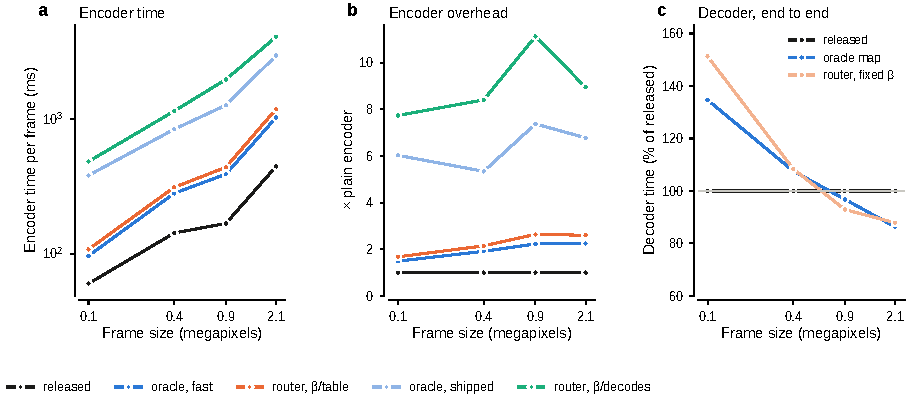
\includegraphics[width=\textwidth]{figs/rt_fig2_resolution.pdf}
\caption{Encoder time (a), encoder overhead (b) and end-to-end decoder time (c) against frame size.}\label{fig:rt_resolution}\end{figure*}
\begin{figure*}[t]\centering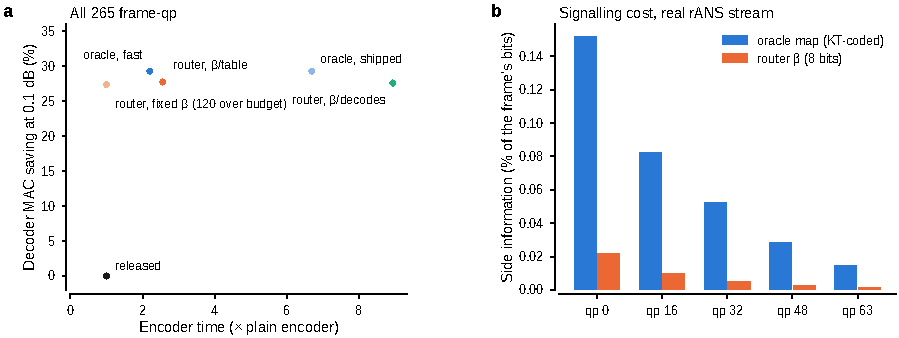
\includegraphics[width=\textwidth]{figs/rt_fig3_tradeoff.pdf}
\caption{Decoder MAC saving against encoder overhead (a) and side information as a share of the real bitstream (b).}\label{fig:rt_tradeoff}\end{figure*}
\begin{figure*}[t]\centering\includegraphics[width=\textwidth]{figs/rt_fig4_image_decoders.pdf}
\caption{Oracle search cost for NoGAN-MS and ELIC (a), saving delivered (b) and decodes per image (c).}\label{fig:rt_image}\end{figure*}
% ---- encoder / decoder runtime (cvpr2027/reports/encoder_runtime) ----
\begin{figure*}[t]\centering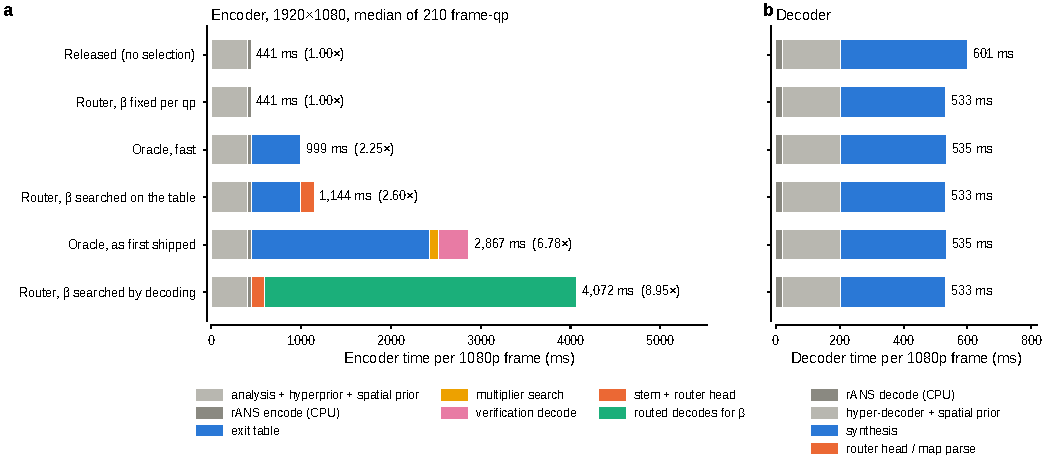
\includegraphics[width=\textwidth]{figs/rt_fig1_timeline_1080p.pdf}
\caption{Encoder (a) and decoder (b) time per 1080p frame for each exit-map selection regime, split into stages (DCVC-UF, CTC).}\label{fig:rt_timeline}\end{figure*}
\begin{figure*}[t]\centering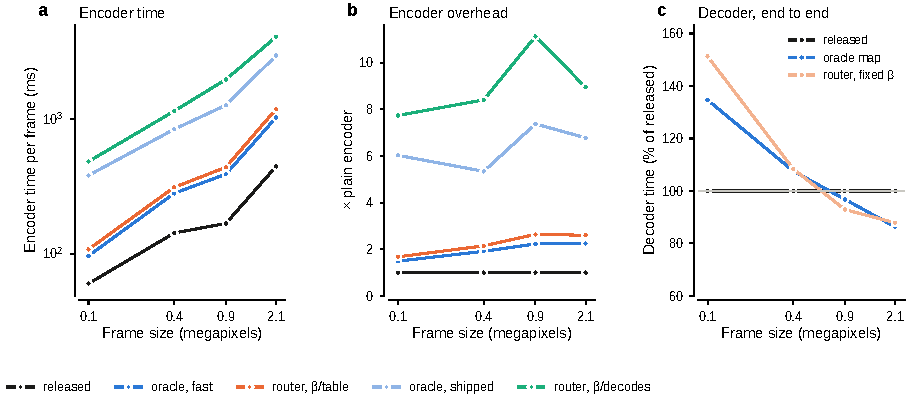
\includegraphics[width=\textwidth]{figs/rt_fig2_resolution.pdf}
\caption{Encoder time (a), encoder overhead (b) and end-to-end decoder time (c) against frame size.}\label{fig:rt_resolution}\end{figure*}
\begin{figure*}[t]\centering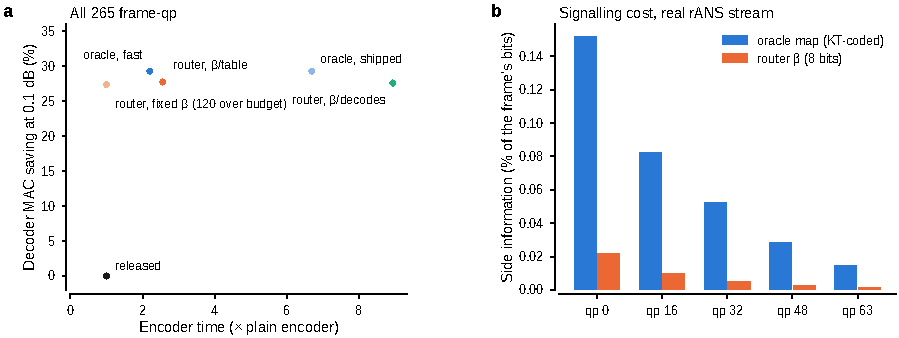
\includegraphics[width=\textwidth]{figs/rt_fig3_tradeoff.pdf}
\caption{Decoder MAC saving against encoder overhead (a) and side information as a share of the real bitstream (b).}\label{fig:rt_tradeoff}\end{figure*}
\begin{figure*}[t]\centering\includegraphics[width=\textwidth]{figs/rt_fig4_image_decoders.pdf}
\caption{Oracle search cost for NoGAN-MS and ELIC (a), saving delivered (b) and decodes per image (c).}\label{fig:rt_image}\end{figure*}
